% !TeX root = RJwrapper.tex
\title{Ordinal Regression Diagnostics in R: An Introduction to the ordr package}
\author{by Brandon M. Greenwell, Author Two and Author Three}

\maketitle

\abstract{
An abstract of less than 150 words.
}


%%%%%%%%%%%%%%%%%%%%%%%%%%%%%%%%%%%%%%%%%%%%%%%%%%%%%%%%%%%%%%%%%%%%%%%%%%%%%%%%
\section{Introduction}
%%%%%%%%%%%%%%%%%%%%%%%%%%%%%%%%%%%%%%%%%%%%%%%%%%%%%%%%%%%%%%%%%%%%%%%%%%%%%%%%

Categorical outcomes are encountered frequently in practice. Oftentimes, the categories are ordered. For example, in an opinon poll, the response may be satisfaction (e.g., $\mathcal{Y} \in \left\{Low, Medium, High\right\}$).

The \dfn{cumulative link} model is a natural choice for modelling an ordinal outcome. Consider an ordinal categorical outcome $\mathcal{Y}$ with ordered categories $1 < 2 < \dots < J$. In a cumulative link model, the cumulative probabilities are linked to the linear predictor according to
\begin{equation}
\label{eqn:clm}
  G^{-1}\left(\Pr\left\{\mathcal{Y} \le j\right\}\right) = \alpha_j + \boldsymbol{\beta}\boldsymbol{X},
\end{equation}
where $G$ is a continuous cumulative distribution function, $\alpha_j$ are the category-specific intercepts, $\boldsymbol{X}$ is a matrix of covariates, and $\boldsymbol{\beta}$ is a vector of fixed regression coefficients. The intercept parameters satisfy $-\infty = \alpha_0 < \alpha_1 < \dots < \alpha_{J-1} < \alpha_J = \infty$. Common choices for the link function $G^{-1}$ include:
\begin{description}
  \item[logit:] $G^{-1}\left(p\right) = \log\left[p / \left(1 - p\right)\right]$;
  \item[probit:] $G^{-1}\left(p\right) = \Phi^{-1}\left(p\right)$ (i.e., the quantile function for the standard normal distribution);
  \item[log-log:] $G^{-1}\left(p\right) = \log\left[-\log\left(p\right)\right]$;
  \item[complimentary log-log:] $G^{-1}\left(p\right) = \log\left[-\log\left(1 - p\right)\right]$;
  \item[cauchit:] $G^{-1}\left(p\right) = \tan\left(\pi p - \pi / 2\right)$.
\end{description}

There a number of R packages that can be used to fit models of the form \eqref{eqn:clm}. The recommended package \CRANpkg{MASS} \citep{pkg-MASS} has the function \code{polr} (proportional odds logistic regression) which can be used with all of the above link functions. The \CRANpkg{VGAM} \citep{pkg-VGAM} package has the \code{vglm} function for fitting \dfn{vector generalized linear models}, which includes the broad class of cumulative link models. Package \CRANpkg{ordinal} \citep{pkg-ordinal} has the \code{clm} function for fitting cumulative link models. The popular \CRANpkg{rms} package \citep{pkg-rms} has two functions: \code{lrm} for fitting logistic regression models which allows the response to be an ordinal factor, and \code{orm} for fitting ordinal regression models of the form \eqref{eqn:clm}.

For a continuous outcome, the residual is traditionally defined as the observed and fitted values. For categorical outcomes, the residuals are more difficult to define.

Very few residuals for ordinal regression models have been proposed in the literature. \citet{graphical-liu-2009} proposed using the cumulative sums of residuals derived from collapsing the ordered categories into multiple binary outcomes. Unfortunately, this method leads to multiple residuals for the ordinal outcome and therefore difficult to interpret. \citet{residuals-li-2012} showed that the sign-based statistic
\begin{equation}
\label{eqn:pres}
  r_{prob} = E\left\{sign\left(y - \mathcal{Y}\right)\right\} = Pr\left\{y > \mathcal{Y}\right\} - Pr\left\{y < \mathcal{Y}\right\},
\end{equation}
can be used as a residual for proportional odds regression models. For an overview of the theoretical and graphical properties of \eqref{eqn:pres}, see \citet{residuals-liu-2017}. These are available in the \CRANpkg{PResiduals} package \citep{pkg-PResiduals}. A limitation of the probability-scale residuals is that they are discrete...


%%%%%%%%%%%%%%%%%%%%%%%%%%%%%%%%%%%%%%%%%%%%%%%%%%%%%%%%%%%%%%%%%%%%%%%%%%%%%%%%
\subsection{Surrogate-based residuals}
%%%%%%%%%%%%%%%%%%%%%%%%%%%%%%%%%%%%%%%%%%%%%%%%%%%%%%%%%%%%%%%%%%%%%%%%%%%%%%%%

The problem with the LS residuals is that they are based on a discrete outcome and hence, discrete themselves. This makes using them in various diagnostic plots far less useful. The surrogate based residual, on the other hand, is based on a continuous (unobserved) latent variable $S$ and is far better suited for use in visual diagnostics.

Proposed in \citet{residuals-liu-2017}.


%%%%%%%%%%%%%%%%%%%%%%%%%%%%%%%%%%%%%%%%%%%%%%%%%%%%%%%%%%%%%%%%%%%%%%%%%%%%%%%%
\subsubsection{Graphical properties}
%%%%%%%%%%%%%%%%%%%%%%%%%%%%%%%%%%%%%%%%%%%%%%%%%%%%%%%%%%%%%%%%%%%%%%%%%%%%%%%%

Coming soon!



%%%%%%%%%%%%%%%%%%%%%%%%%%%%%%%%%%%%%%%%%%%%%%%%%%%%%%%%%%%%%%%%%%%%%%%%%%%%%%%%
\section{Residual-based OR diagnostics in R}
%%%%%%%%%%%%%%%%%%%%%%%%%%%%%%%%%%%%%%%%%%%%%%%%%%%%%%%%%%%%%%%%%%%%%%%%%%%%%%%%

The \pkg{ordr} package currently only exports three functions:
\begin{description}
  \item[\code{resids}] construct (surrogate-based) residuals for fitted model objects of class \code{"clm"}, \code{"polr"}, and \code{"vglm"};
  \item[\code{autoplot}] produce various diagnostic plots using \CRANpkg{ggplot2} graphics \citep{pkg-ggplot2};
 \item[\code{gof}] - simulate p-values from a goodness-of-fit test.
\end{description}

For illustration, we generated $n = 2000$ observations from the following ordered probit model:
\begin{equation}
\label{eqn:quadratic}
  Pr\left\{\mathcal{Y} \le j\right\} = \Phi\left\{\left(\alpha_j + \beta_1 X + \beta_2 X ^ 2\right)\right\}, \quad j = 1, 2, 3, 4,
\end{equation}
where $\alpha_1 = -16$, $\alpha_2 = -12$, $\alpha_3 = -8$, $\beta_1 = 8$, $\beta_2 = -1$, and $X \sim \mathcal{U}\left(1, 7\right)$. These simulated data are available in the \code{df.quadratic} data frame from the \pkg{ordr} package. Below, we fit a (correctly specified) probit model using the \code{polr} function from the \pkg{MASS} package.
\begin{example}
  library(MASS)
  data(df.quadratic, package = "ordr")
  fit.polr <- polr(y ~ x + I(x ^ 2), data = df.quadratic, method = "probit")
\end{example}

The code chunk below obtains the probability-scale residuals \eqref{eqn:pres} from the previously fitted probit model \code{fit.polr} using the \pkg{PResiduals} package.
\begin{example}
  library(PResiduals)
  pres <- presid(fit.polr)  # probability-scale residuals
\end{example}
A couple diagnostic plots based on these residuals are shown in the bottom row of \ref{fig:correct-model}. (\strong{Note:} the reference distribution for the probability-based residual is the $\mathcal{U}\left(-1, 1\right)$ distribution.) As can be seen, these residuals, which are inherently discrete, often display unusual patterns in diagnostic plots, making them less useful as a diagnostic tool for ordinal regression models.

Similarly, we can use the \code{resids} function in package \code{ordr} to obtain the surrogate-based residuals. This is illustarted in the following code chunk. the results are displayed in the top row of Figure~\ref{fig:correct-model}. (Since \pkg{ggplot2} has already been loaded, we can just use \code{autoplot}.)
\begin{example}
  library(ordr)
  sres <- resids(fit.polr)

  # Figure 1 (top)
  p1 <- autoplot(sres, what = "covariate", x = df.quadratic$x) +
    xlab("x")
  p2 <- autoplot(sres, what = "qq", distirbution = pnorm)

  # Figure 1 (bottom)
  p3 <- ggplot(data.frame(x = df.quadratic$x, y = pres), aes(x, y)) +
    geom_point(alpha = 0.5) +
    geom_smooth(color = "red", se = FALSE) +
    ylab("Probability residual")
  p4 <- ggplot(data.frame(y = pres), aes(sample = y)) +
    stat_qq(distribution = qunif, dparams = list(min = -1, max = 1), alpha = 0.5) +
    xlab("Sample quantile") +
    ylab("Theoretical quantile")

  # Figure 1
  grid.arrange(p1, p2, p3, p4, ncol = 2)
\end{example}
Alternatively, we wrote methods for various ordinal regression model classes, so you can just give \code{autoplot} the fitted model directly. The benefit of this approach is that the reference distirbution is automatically extracted.
\begin{example}
  autoplot(fit.polr, what = "qq")  # same as top right of Figure 1
\end{example}

\begin{figure}[!htbp]
  \centering
  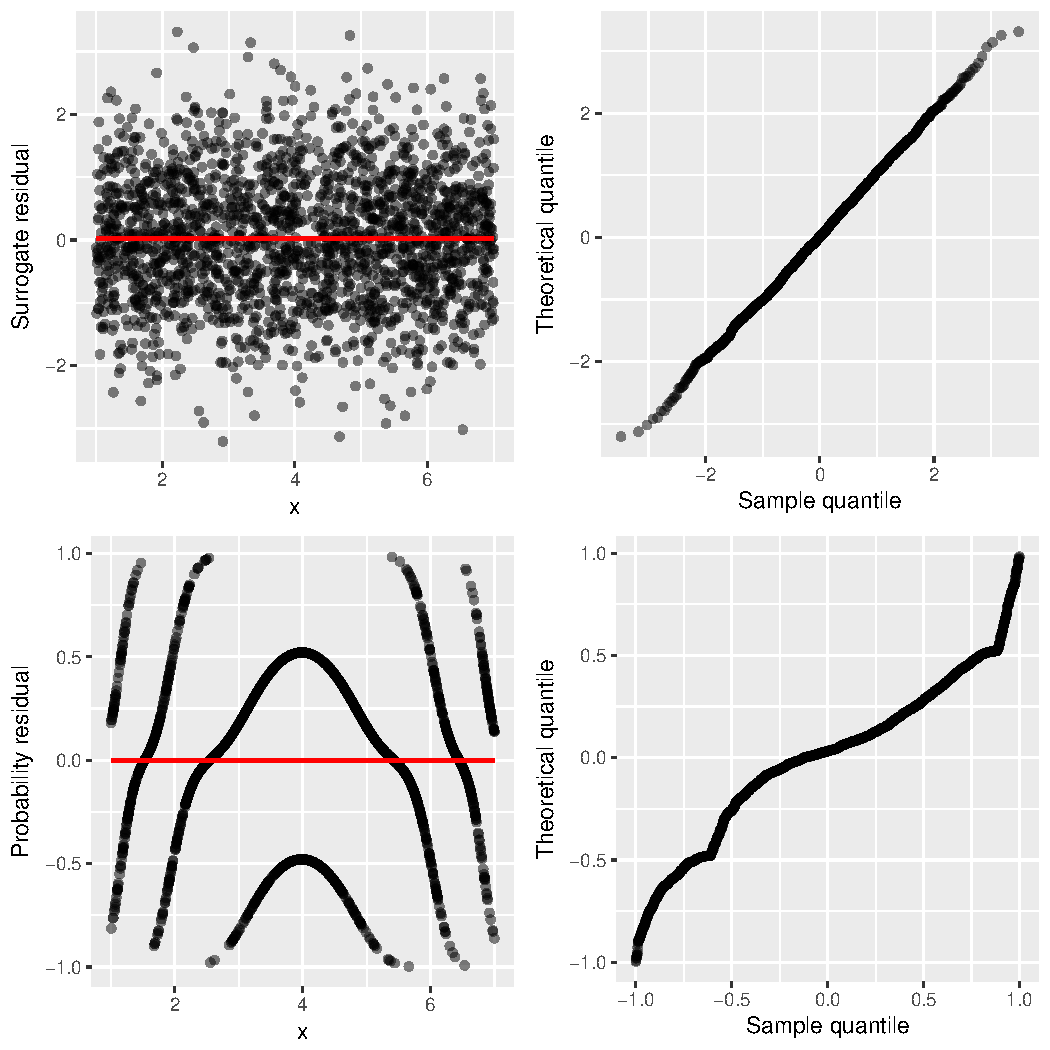
\includegraphics[width=1\textwidth]{correct-model}
  \caption{Various diagnostic plots for a (correctly specified) probit model fit to the simulated data from model \eqref{eqn:quadratic}. \textit{Top left}: Surrogate residual vs. covariate plot. \textit{Top right}: Quantile-quantile plot of the surrogate residuals. \textit{Bottom left}: Probability-scale residual vs. covariate plot. \textit{Bottom right}: Quantile-quantile plot of the probability-scale residuals.}
  \label{fig:correct-model}
\end{figure}


%%%%%%%%%%%%%%%%%%%%%%%%%%%%%%%%%%%%%%%%%%%%%%%%%%%%%%%%%%%%%%%%%%%%%%%%%%%%%%%%
\subsection{Detecting a misspecified mean structure}
%%%%%%%%%%%%%%%%%%%%%%%%%%%%%%%%%%%%%%%%%%%%%%%%%%%%%%%%%%%%%%%%%%%%%%%%%%%%%%%%

Suppose that we did not include the quadratic term in our fitted model. We could expect a residual-vs-$x$ plot to clearly indicate that such a (correct) quadratic term is missing...
The probability-scale residual gives some indication of a misspecified mean structure, but this only becomes more clear with increasing $J$ and the plot is still discrete. This is oversome by the surrogate residuals which produces a residual plot not unlike those seen in ordinary linear regresion models...

\begin{example}
  fit.polr <- update(fit.polr, y ~ x)  # remove quadratic term
\end{example}



\begin{figure}[!htbp]
  \centering
  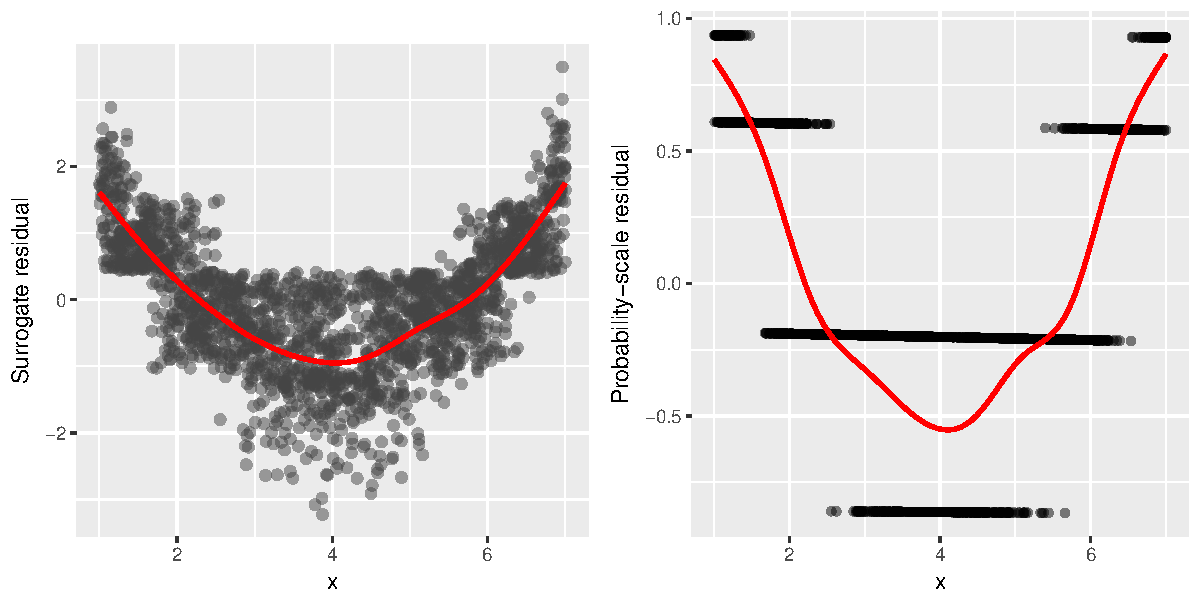
\includegraphics[width=1\textwidth]{quadratic}
  \caption{Various diagnostic plots for a probit model with a misspecified mean structure fit to the simulated data from model \eqref{eqn:quadratic}. \textit{Left}: Surrogate residual vs. covariate plot. \textit{Right}: Probability-scale residual vs. covariate plot.}
  \label{fig:quadratic}
\end{figure}


%%%%%%%%%%%%%%%%%%%%%%%%%%%%%%%%%%%%%%%%%%%%%%%%%%%%%%%%%%%%%%%%%%%%%%%%%%%%%%%%
\subsection{Detecting heteroscedasticty}
%%%%%%%%%%%%%%%%%%%%%%%%%%%%%%%%%%%%%%%%%%%%%%%%%%%%%%%%%%%%%%%%%%%%%%%%%%%%%%%%

For this example, we generated $n = 2000$ observations from the following ordered probit model:
\begin{equation*}
  Pr\left\{\mathcal{Y} \le j\right\} = \Phi\left\{\left(\alpha_j + \beta X\right) / \sigma_X\right\}, \quad j = 1, 2, 3, 4, 5,
\end{equation*}
where $\alpha_1 = -36$, $\alpha_2 = -6$, $\alpha_3 = 34$, $\alpha_4 = 64$, $\beta = -4$, $X \sim \mathcal{U}\left(2, 7\right)$, and $\sigma_X = X ^ 2$.

The following block of code uses the \pkg{MASS} package function \code{polr} to fit a probit model to the \code{hd} data.
\begin{example}
  library(ggplot2)
  library(MASS)
  library(ordr)
  fit.polr <- polr(y ~ x, data = hd, method = "probit")
  set.seed(101)  # for reproducibility
  sur.res <- resids(fit.polr)  # surrogate-based residuals

  # Figure 1 (left)
  ggplot(data.frame(x = hd$x, y = sur.res), aes(x, y)) +
    geom_point(size = 2, alpha = 0.25) +
    geom_smooth(color = "red", se = FALSE) +
    ylab("Surrogate residual")
\end{example}
Alternatively, we can plot the residuals directly from the fitted model using the \code{autoplot} function:
\begin{example}
  autoplot(fit.polr, what = "covariate", x = hd$x)  # plot not shown
\end{example}

We can also easily obtain and plot the standard Li-Shepherd residuals against $x$ using the \pkg{PResiduals} package function \code{presid}:
\begin{example}
  library(PResiduals)
  ls.res <- presid(fit.polr)  # probability-scale residuals

  # Figure 1 (right)
  ggplot(data.frame(x = hd$x, y = ls.res), aes(x, y)) +
    geom_point(size = 2, alpha = 0.25) +
    geom_smooth(color = "red", se = FALSE) +
    ylab("probability-scale residual")
\end{example}

In this case, it is less clear that there is an issue with constant variance from the probability-scale residual plot...

\begin{figure}[!htbp]
  \centering
  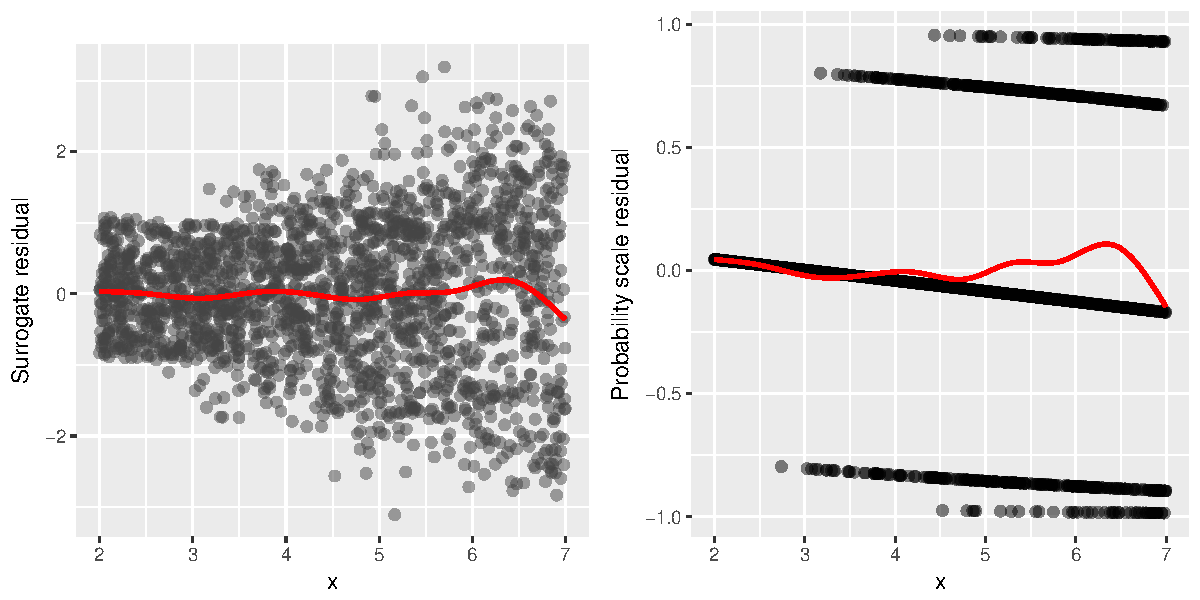
\includegraphics[width=1\textwidth]{heteroscedasticity}
  \caption{Residual vs. covariate plots for the simulated heteroscedastid data. \textit{Left}: Surrogate residuals. \textit{Right}: probability-scale residuals.}
  \label{fig:heteroscedasticity}
\end{figure}


%%%%%%%%%%%%%%%%%%%%%%%%%%%%%%%%%%%%%%%%%%%%%%%%%%%%%%%%%%%%%%%%%%%%%%%%%%%%%%%%
\subsection{Detecting a misspecified link function}
%%%%%%%%%%%%%%%%%%%%%%%%%%%%%%%%%%%%%%%%%%%%%%%%%%%%%%%%%%%%%%%%%%%%%%%%%%%%%%%%

Coming soon!


%%%%%%%%%%%%%%%%%%%%%%%%%%%%%%%%%%%%%%%%%%%%%%%%%%%%%%%%%%%%%%%%%%%%%%%%%%%%%%%%
\subsection{Checking the proportionality assumption}
%%%%%%%%%%%%%%%%%%%%%%%%%%%%%%%%%%%%%%%%%%%%%%%%%%%%%%%%%%%%%%%%%%%%%%%%%%%%%%%%

Coming soon!


%%%%%%%%%%%%%%%%%%%%%%%%%%%%%%%%%%%%%%%%%%%%%%%%%%%%%%%%%%%%%%%%%%%%%%%%%%%%%%%%
\subsection{Assessing goodness-of-fit}
%%%%%%%%%%%%%%%%%%%%%%%%%%%%%%%%%%%%%%%%%%%%%%%%%%%%%%%%%%%%%%%%%%%%%%%%%%%%%%%%

Coming soon!

\begin{example}
  plot(gof(houses.polr, nsim = 1000))
\end{example}


%%%%%%%%%%%%%%%%%%%%%%%%%%%%%%%%%%%%%%%%%%%%%%%%%%%%%%%%%%%%%%%%%%%%%%%%%%%%%%%%
\section{Bitterness of wine}
%%%%%%%%%%%%%%%%%%%%%%%%%%%%%%%%%%%%%%%%%%%%%%%%%%%%%%%%%%%%%%%%%%%%%%%%%%%%%%%%

\begin{example}
  library(ordinal)
  data(wine, package = "ordinal")
  wine.clm <- clm(rating ~ temp * contact, data = wine)  # default logit link
\end{example}

\begin{example}
set.seed(101)  # for reproducibility
grid.arrange(
  autoplot(wine.clm, nsim = 10, what = "qq"),
  autoplot(wine.clm, nsim = 10, what = "fitted"),
  autoplot(wine.clm, nsim = 10, what = "cov", x = wine$temp),
  autoplot(wine.clm, nsim = 10, what = "cov", x = wine$contact),
  ncol = 2
)
\end{example}



%%%%%%%%%%%%%%%%%%%%%%%%%%%%%%%%%%%%%%%%%%%%%%%%%%%%%%%%%%%%%%%%%%%%%%%%%%%%%%%%
\section{Summary}
%%%%%%%%%%%%%%%%%%%%%%%%%%%%%%%%%%%%%%%%%%%%%%%%%%%%%%%%%%%%%%%%%%%%%%%%%%%%%%%%

This file is only a basic article template. For full details of \emph{The R Journal} style and information on how to prepare your article for submission, see the \href{https://journal.r-project.org/share/author-guide.pdf}{Instructions for Authors}.


%%%%%%%%%%%%%%%%%%%%%%%%%%%%%%%%%%%%%%%%%%%%%%%%%%%%%%%%%%%%%%%%%%%%%%%%%%%%%%%%
\section{Acknowledgments}
%%%%%%%%%%%%%%%%%%%%%%%%%%%%%%%%%%%%%%%%%%%%%%%%%%%%%%%%%%%%%%%%%%%%%%%%%%%%%%%%

TBD.


\bibliography{greenwell-lastname2-lastname3}

\address{Author One\\
  Affiliation\\
  Address\\
  Country\\
  (ORCiD if desired)\\
  \email{author1@work}}

\address{Author Two\\
  Affiliation\\
  Address\\
  Country\\
  (ORCiD if desired)\\
  \email{author2@work}}

\address{Author Three\\
  Affiliation\\
  Address\\
  Country\\
  (ORCiD if desired)\\
  \email{author3@work}}
